\documentclass[aps,prl,twocolumn,showpacs,superscriptaddress,groupedaddress]{revtex4-1}  % for review and submission
%\documentclass[aps,preprint,showpacs,superscriptaddress,groupedaddress]{revtex4-1}  % for double-spaced preprint
\usepackage[english]{babel}
\usepackage{graphicx}% Include figure files
\begin{document} 
\title{Superabsorption of light by nanoparticles}

% Proposed reviewers: Anatoly Zayats, Andrea Alu, Sergei Bozhevolnyi
% Prof. García de Abajo (http://garciadeabajos-group.icfo.es/)
%  Andrea Alu.
\author{Konstantin Ladutenko} \email[e-mail: ]{k.ladutenko@metalab.ifmo.ru}
\affiliation{ITMO University, 49 Kronverskii Ave., St.~Petersburg
  197101, Russian Federation}

\affiliation{Ioffe Physical-Technical Institute of the Russian Academy
  of Sciences, 26 Polytekhnicheskaya Str., St.~Petersburg 194021,
  Russian Federation}

\author{Pavel Belov} \affiliation{ITMO University, 49 Kronverskii
  Ave., St.~Petersburg 197101, Russian Federation}

\author{Ovidio Pe\~{n}a-Rodr\'{i}guez} \affiliation{Instituto de
  Fusi\'{o}n Nuclear, Universidad Polit\'{e}cnica de Madrid, Jos\'{e}
  Guti\'{e}rrez Abascal 2, E-28006 Madrid, Spain}

\author{Ali Mirzaei} \author{Andrey Miroshnichenko} \author{Ilya
  Shadrivov} \affiliation{Nonlinear Physics Centre, Research School of
  Physics and Engineering, The Australian National University, 59
  Mills Rd, Acton, ACT, 2601, Australia}

\date{\today}
\begin{abstract}
  Nanoparticles have a fundamental limit as to how much light they can
  absorb. This limit is based on the finite number of modes excited
  in the nanoparticle at a given wavelength and maximum absorption
  capacity per mode. The enhanced absorption can be achieved when each
  mode supported by the nanopartice absorbs light up to the maximum
  capacity. Using stochastic optimization algorithm, we design
  multilayer nanoparticles, in which we can make several resonant
  modes overlap at the same frequency resulting in {\it
    superabsorption}.  We further introduce the {\it efficiency of the
    absorption} for a nanoparticle, which is the absorption normalized
  by the physical size of the particle, and show that efficient
  absorbers are not always operating in the superabsorbing regime.
\end{abstract}


\pacs% insert suggested PACS numbers in braces on next line,
% not more that 4
{41.20.Jb 42.25.Bs 02.60.Pn 02.70.-c}
% 41.20.Jb Electromagnetic wave propagation
%% 42.25.Bs Wave propagation, transmission and absorption
%% 02.60.Pn Numerical optimization
% 02.70.-c Computational techniques; simulations

\maketitle %\maketitle must follow title, authors, abstract and \pacs

Mie theory~\cite{Mie-1908}, which is over 100 years old, describes
interaction of electromagnetic waves with spherical particles. Mie
solution is still of great interest these
days~\cite{Suzuki-2008,MacKowski-2012,Lerme-2000,Xu-2005,Li-2006,Gogoi-2010,Santiago-2011},
since it is one of the primary tools for analyzing wave scattering by
spherical objects. Further development of the Mie
theory~\cite{Yang-2003, Pena-scattnlay-2009} made it possible to apply
it to the study of multilayer spherical
particles~\cite{Sheehan-2013,Selmke-2012}.  Such particles have
various applications in cancer treatment~\cite{Zhang-2010,
  Hirsch-2003}, medical diagnostics~\cite{Allain-2002},
cloaking~\cite{Qui-2009, Semouchkina-2013, Ladutenko-2014} and
plasmonic devices~\cite{Martin-2013, Alu-2005}, in the study of
thermal properties of insulating materials~\cite{Xie-2013}, as well as
for improving solar cells performance~\cite{Kameya-2011,Mann-2011}.

The scattering properties of multilayer cylinders and spheres was
studied in great detail by Ruan and Fan~\cite{Fan-2010,Fan-2011}.  In
these works the authors introduced the concept of superscattering,
when scattering cross-section of a multilayer particle exceeds that of
a homogeneous particle of the same size in the so-called
single-channel limit. Superscattering appears when a multilayer
structure has several nearly degenerate modes, i.e. their resonance
frequencies coincide or are close to each other. In a homogeneous
particle, resonances appear at different frequencies, and there is no
design freedom to make these resonances overlap, and this limits the
achievable scattering cross-section.

Similar fundamental limitations exist for the absorbing properties of
subwavelength nanoparticles.  Tribelsky~\cite{Tribelsky-2011} has
derived a theoretical limit of a maximum absorption cross-section
(ACS) value for a single channel, i.e., when only one mode of a sphere
is excited.  As a result, the absorption coefficients $\tilde{a}_n=
{\rm Re}\{a_n\} - |a_n|^2 $ and $\tilde{b}_n= {\rm Re}\{b_n\} -
|b_n|^2 $ become limited by $1/4$, here $a_n$ and $b_n$ are scattering
coefficient as defined within the Mie theory~\cite{Bohren-1983} for
expansion of the scattered electric field:
$$ 
 {\rm \mathbf{E}}_s = \sum_{n=1}^{\infty} E_n
 \left(
   i a_n {\rm \mathbf{N}}_{e1n}^{(3)} - b_n{\rm\mathbf{M}_{o1n}^{(3)}}
 \right),
$$
where ${\rm \mathbf{N}}_{e1n}^{(3)}$ and ${\rm\mathbf{M}_{o1n}^{(3)}}$
are corresponding vector spherical harmonics,
$E_n=i^nE_0(2n+1)/n(n+1)$, $n$ is the angular momentum of the mode,
and $E_0$ is the amplitude of the incident field.

To overcome these limitations, we employ similar approach to the one
used for enhancing scattering cross-section~\cite{Fan-2011}. In
particular, we propose to use the multilayer structures, and by means
of stochastic optimization algorithm~\cite{Jingqiao-JADE-2009} we
optimize the ACS of such nanoparticles. We analyze the absorption
cross-section of these particles, and present the superabsorption
regime. We further introduce the absorption efficiency, which is the
ACS normalized to the geometric cross-section of particles. Here we
show that there is a strong counterplay between the increased
absorption for larger particles vs size for smaller particles, and
quite remarkably we find that the most {\em efficient} absorption can
be achieved in a single channel limit for small particles.

Another approach for an ideal absorber is given in the recent work by
Grigoriev et al.~\cite{Grigoriev-2015}. Authors considered only dipole
approximation, and the final result is very close to the dipole limit
predicted by Tribelsky~\cite{Tribelsky-2011}.  Such absorption design
corresponds to the single mode limit.  At the same time, Grigoriev et
al.~\cite{Grigoriev-2015} also provide an equation to design a
core-shell structure from given materials. However, in the case of
$Si$ core and $Ag$ shell materials and sizes taken from the best
design obtained in the present paper, their equation gives a complex
value for the core material filling factor, which cannot be achieved
in experimental realisations.

\begin{figure}
  \center{
    % Use pdfcrop to remove white margins
    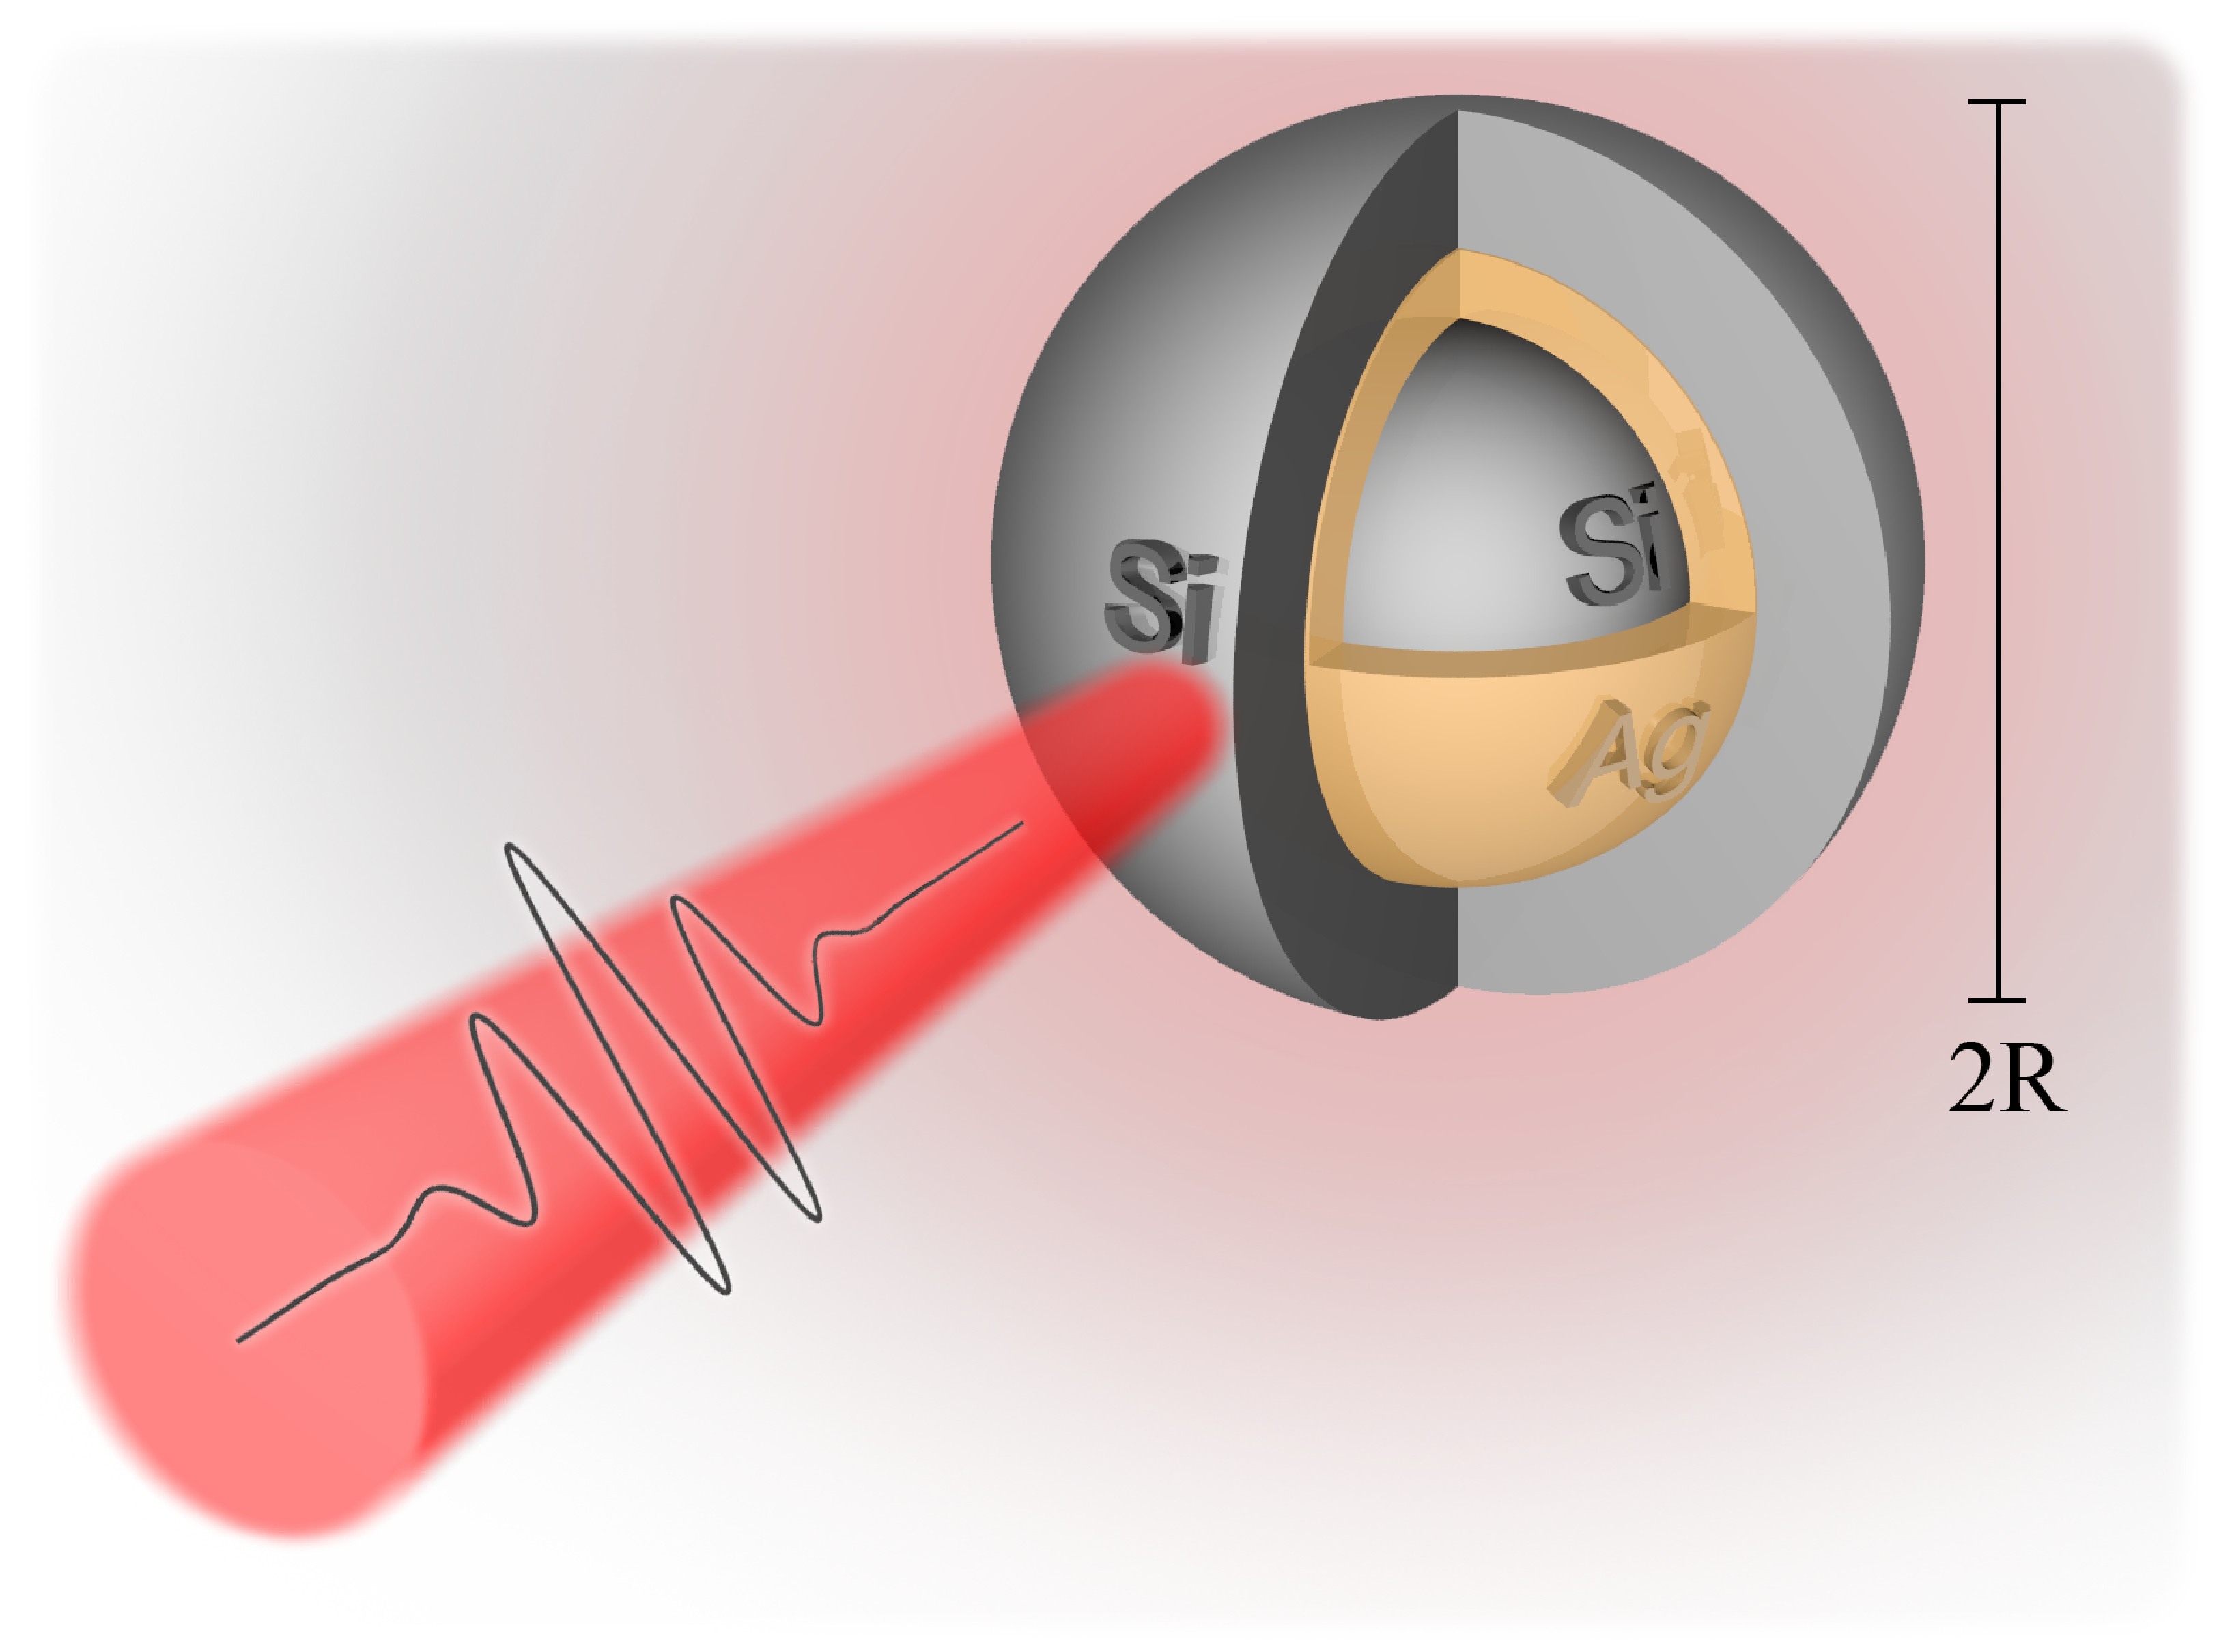
\includegraphics[width=0.4\textwidth]{fig/Fig1}%
    \caption{(color online) Shematic view of the simulated $Si/Ag/Si$ particle. 
      \label{fig:geom}
    }%
  }
\end{figure}

The proposed approach can be applied to arbitrary combination of materials, but to be more specific in what follows we
consider dielectric-metal-dielectric triple-layer $Si/Ag/Si$
spherical particle illuminated by a plane wave schematically shown
in Fig.~\ref{fig:geom}. In what follows we describe the materials
using experimentally measured parameters from Ref.~\cite{palik-1997},
and, e.g. at $\lambda = 500$ nm $\epsilon_{Si} = 18.5 + i0.63$ and
$\epsilon_{Ag} = -8.5 + i0.76$.  To optimize the thickness of each
layer we implemented~\cite{JADE-web} an adaptive differential
evolution algorithm~\cite{Storn-DE-first-1997}, which is called
JADE~\cite{Jingqiao-JADE-2009}.  The technical details of the
optimization algorithm were published previously in
Ref.~\cite{Ladutenko-2014}. We perform Mie calculations using the
Scattnlay software~\cite{Pena-scattnlay-2009,Scattnlay-web}, whose
results are verified by a number of other implementations of the Mie
solutions and by commercially available software including CST
Microwave studio~\cite{CST-web} and Comsol
Multiphysics~\cite{Comsol-web}.

It is a common understanding that, in general, a larger particle has a
larger absorption cross-section, so sphere with the diameter of 1 cm
absorbs more light than any nanoscale sphere. Therefore, it is
practical to employ {\em the absorption efficiency} $Q_{\rm
  abs}=C_{\rm abs}/\pi R^2$, where $R$ is the outer radius of the
particle and $C_{\rm abs}$ is the absorption cross-section.

\begin{figure}
  \center{
    % Use pdfcrop to remove white margins
    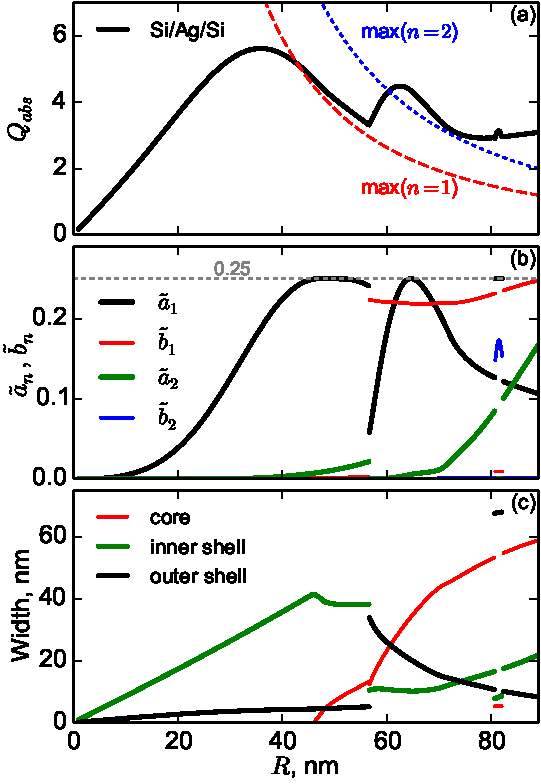
\includegraphics[width=0.45\textwidth]{fig/2015-04-01-Qabs-SiAgSi-overview}%
    \caption{(color online) Results of optimization of the absorption efficiency
      for the fixed wavelength of 500~nm. (a) Absorption efficiency
      with the best value achieved for the particle of the double-layer Ag/Si design of the radius of 36~nm. Dashed lines show theoretical
      limits for the first channel and second channel
      absorption. The second and third peaks in the absorption efficiency
      curve exceed the theoretical limit for the second mode
      absorption at $R=63$~nm and $R=81$~nm. Local maxima of
      absorption efficiency are additionally marked with arrows. (b) Mie absorption
      coefficients for individual excited modes of the optimized
      structures. (c) Optimized layer thicknesses. For the total
      particle radius below 46~nm the optimizer converges to
      a bi-layer structure, when core size vanishes, and the
      optimum design is a $Ag/Si$ particle. 
      \label{fig:overview}
    }%
  }
\end{figure}
%
In order to study the dependence of the absorption efficiency on the
outer particle size, we run optimization algorithm for different
(fixed) particle outer size, and our optimization parameters are the
radii of internal cores, whereas the target function is the absorption
efficiency. We maximize absorption efficiency at a fixed wavelength of
the incident light (we have chosen $\lambda=500$~nm). We show the
results of our stochastic optimization algorithm in
Fig.~\ref{fig:overview}~(a).  Dashed lines show theoretical absorption
limit of a dipole ($n=1$) and a quadrupole ($n=2$)
resonances~\cite{Tribelsky-2011}, which are given as $$Q^{(n)}_{\rm
  abs\ max}=\frac{2n+1}{2q^2},$$ where the size parameter $q=2\pi
R/\lambda$, and $n$ is the angular momentum of the mode. Following
Ref.~\cite{Fan-2011}, where the authors introduce superscattering for
spherical particles, here we introduce superabsorption regime, when
{\em the ACS is larger than the theoretical limit for absorption by
  strongly excited mode with the highest angular momentum $n$}. In our
parameter space we have modes up to the quadrupole excited
($n=2$), and in order to get superabsorption our efficiency should be
higher than that of a quadrupole. We clearly see this superabsorption
regime at $R>60$~nm, in Fig.~\ref{fig:overview}~(a).

In Fig.~\ref{fig:overview}~(b) we present the values of Mie absorption
coefficients for individual excited modes in the structure, while
horizontal dashed line shows the theoretical limit (1/4) for each of
them. $\tilde{a}_{1,2}$ are electric dipole and electric quadrupole,
while $\tilde{b}_{1,2}$ are magnetic dipole and magnetic
quadrupole. For small particles, as expected, absorption is dominated
by electric dipole $\tilde{a}_1$.  At $R > 56.6$~nm the optimization
procedure finds that the designs with both electric and magnetic
dipoles have larger ACS than the structure with only the electric
dipole excited. This is why the curves in
Figs.~\ref{fig:overview}~(b,c) experience the discontinuity. Quite remarkably, in this regime, {\em the combined absorption of the electric and magnetic dipoles exceeds the theoretical limit for the higher order (quadrupole) mode.}  We also
note that there is a very narrow range of particle sizes, between
80.7~nm and 82.1~nm, where our analysis finds that the design
supporting electric dipole $\tilde{a}_1$ and magnetic quadrupole
$\tilde{b}_2$ has larger ACS, and this explains two more
discontinuities of the curves at the respective size values.

Fig.~\ref{fig:overview}~(c) shows optimized sizes of layers inside a
multilayer structure. It reveals quite a curious result, that the
dipole branch (i.e. for particle radii below 56.6~nm) has two
parts. For $R<46$~nm the best absorber has just two layers, as the
radius of the core of a triple-layer structure vanishes, and the
particle reduces to $Ag/Si$ core-shell structure.  At $R=46$~nm dipole
channel reaches its theoretical limit (it becomes
$\tilde{a}_1>0.249$).  It appears that the optimizer introduced the
inner $Si$ layer in order to keep $\tilde{a}_1$ near the theoretical
limit as the $R$ increases.  As a side effect, the quadrupole
contribution $\tilde{a}_2$ appears; however, it does not help to reach
superabsorption limit for $n=2$.

Remarkably, the absolute maximum {\em absorption efficiency} is not
reached within the superabsorption regime. Figure~\ref{fig:overview}
shows that the maximum efficiency is achieved for small particle size,
and the ACS is still well below the single channel limit. It appears
that the $Ag/Si$ core-shell nanoparticle with the total radii of
approximately 36~nm is the most efficient absorber among the considered
structures, whose ACS reaches values {\em over 5 times the physical
  cross-section area of the particle}.  From a practical point of view,
it is quite important that the maximum can be reached in a bi-layer
structure, instead of a triple-layer, since it should be easier and
cheaper to fabricate.

\begin{figure}
  \center{
    % Use pdfcrop to remove white margins
    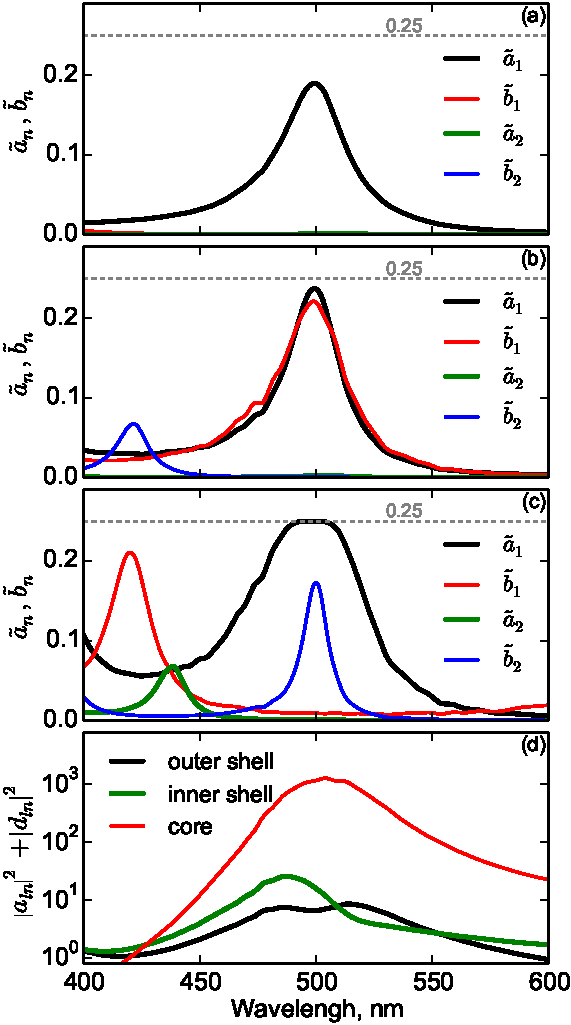
\includegraphics[width=0.45\textwidth]{fig/2015-04-01-SiAgSi-ab-spectra4}%
    \caption{(color online) Spectra of Mie absorption coefficients of (a) efficient and (b-c)superabsorption design. Panel (d) shows the superposition of the squared absolute values of the Mie coefficients for electric dipole contribution inside each layer. 
      \label{fig:spectra}
    }%
  }
\end{figure}
To study spectral properties of structures with large ACS which we
obtained by the optimization, in Fig.~\ref{fig:spectra} we plot three
different cases for designs that correspond to local maxima of $Q_{\rm
  abs}$ shown in Fig.~\ref{fig:overview}~(a).  As expected, the design
corresponding to the maximum absorption efficiency at $R=36$~nm has a
single electric dipole resonance centered at the target wavelength
$\lambda=500$~nm. Spectra of designs with maxima at $R=63$~nm and
$R=81$~nm have a signature of the superabsorption, i.e. there is an
overlap of several resonances.  We note that these structures have
additional absorption resonances, but they are located far from the
wavelength of interest.  A noticeable feature of
Fig.~\ref{fig:spectra}~(c) is an almost flat top of the electric
dipole resonance. More detailed analysis shows that we have {\em
  excited several electric dipole resonances} with close resonance
frequencies within our multilayer structure. Indeed, if we plot a
superposition of the squares of the absolute values of the Mie
coefficients, which characterize electric energy density stored in each layer, we find
that we excite resonances in all three layers, and they are slightly
offset as shown in Fig.~\ref{fig:spectra}~(d). Combined effect of
these resonances produces the flat and relatively broadband electric
resonance response shown in Fig.~\ref{fig:spectra}~(c).

\begin{figure}
  \center{
    % Use pdfcrop to remove white margins
    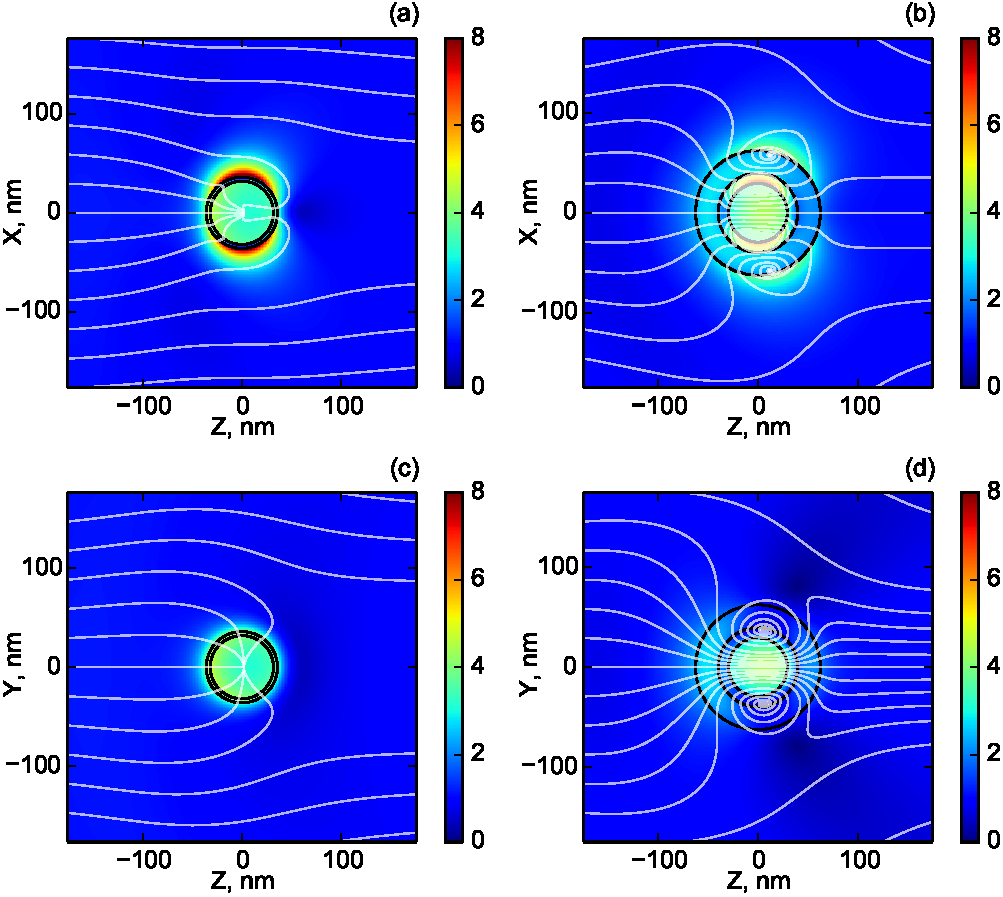
\includegraphics[width=0.47\textwidth]{fig/SiAgSi-flow-R62-YZ-Eabs}%
    \caption{(color online) Amplitude of electric field for $R=36$~nm (a,c) and
      superabsorbing designs (b,d) in E-k  (a-b) and H-k (c-d)
      planes normalized to incident wave.  White curves show the
      energy flow streamlines, plane wave comes from the left.
      \label{fig:field}
    }%
  }
\end{figure}
Finally, we present distribution of the amplitude of the electric
field in Fig.~\ref{fig:field} for two designs: with the best
efficiency at $R=36$~nm and in a superabsorbing design with $R=63$~nm.
Using semi-transparent white curves we also plot streamlines of the
Poynting vector which characterize energy flow.  For the effective
design of the absorber, the power from a large cross-sectional area
flows into the particle.  In case of superabsorption regime, we
observe the formation of vortices in the power flow, which make
absorption more efficient as the electromagnetic energy propagates
several times through the absorbing materials.  The reason for the
smaller overall absorption efficiency of a superabsorbing design is
obvious: spatial distribution of the electric field is not uniform
inside the particle and the share of the volume with high absorption
rate in the vortices does not compensate low absorption efficiency in
the regions with small electric field (absorbed power is expressed as
$P_{\rm abs}=\frac{1}{2}\int\sigma \left|E\right|^2dx\,dy\,dz$)

The stochastic algorithm utilized in our approach is very generic and
the optimization can be repeated for any desired wavelength or
wavelength range.  As a result, one can design spectrally-selective
absorbers or broadband absorbers with almost arbitrary prescribed
properties. We note, that using this algorithm, one can optimize not only absorbtion efficiency, but also other parameters that may be desired for some applications. As an example we reproduce some of the results from
the work of Estakhri and Al\`u~\cite{Alu-2014}, where authors aim to design absorbers with small scattering cross-section, and we provide a number of new optimized designs. The efficiency in the Ref.~\cite{Alu-2014} is defined as the ACS normalized to scattering cross-section. Initially, we set the total value of the absorbed power with cross-section of $\alpha_{\rm abs}=\frac{3\lambda^2}{8\pi}$ and
keep the outer radius of the particle fixed. In this case the optimization
gives a result similar to the structure with contributing harmonics
TM${_1}$ and TE$_1$ from Ref~\cite{Alu-2014}.  For $\epsilon_1 =
1.29+i0.01$, $\epsilon_2 = -10.37+ i0.35$, and $\epsilon_3=8.4+i2.33$
as material parameters we obtained radii $\{a_{c1},a_{c2},a_3\}=\{0.142,0.166,0.194\}\lambda$ and
scattering-normalized absorption efficiency $\eta_{\rm abs}^{(\alpha)}
=7.65$ which corresponds to $\eta_{\rm abs}^{(\alpha)} =7.1$
from the original work~\cite{Alu-2014}.  However, if we set the optimizer to keep high level of absoption efficiency $Q_{\rm abs} \approx 5$ the particle becomes much smaller and the size of the outer layer vanishes $\{a_{c1},a_{c2}\}=\{0.00635,0.00747\}\lambda$ resulting in $\eta_{\rm abs}^{(Q)} =544$.  It means that this small particle still absorbs five times its phisical size with a very large scattering-normalized absorption efficiency. 

%Moreover, it is easy to
%set the optimizer to keep $\eta_{\rm abs} \approx 100$ or $\eta_{\rm abs}
%\approx 1000$, resulting $\{a_{c1},a_{c2}\}=\{0.0112,0.0131\}\lambda$,
%$Q_{\rm abs} = 8.65$ or $\{a_{c1},a_{c2}\}=\{0.0052,0.0061\}\lambda$,
%$Q_{\rm abs} = 3.26$ respectively.


In conclusion, we introduce and study the effect of superabsorption,
when the absorption cross-section of the nanoparticle can reach the
theoretical limit for several modes at the same frequency. This
becomes possible when several resonant modes of the structure overlap
at the same frequency, and this regime can be achieved in multilayer
nanoparticles. Moreover, quite unexpectedly we find that the most
efficient absorbers, which are characterized by enhanced absorption
efficiencies, are smaller nanoparticles working in a single mode
regime. We present their spectral characteristics and field structure.
  It is interesting to note that a similar conclusion was
made by Miller et al.~\cite{Miller-2014} for extinction of arbitrary
particles: small size with only dipole response is preferable for
geometric volume normalized efficiency.


\begin{acknowledgments}
  Thanks to David A. Powell for his contribution to the analysis of
  the spectrum feature.  AEM and IVS acknowledge the support
  from the Australian Research Council through Future Fellow and
  Discovery project schemes. OPR is grateful to Consejo Nacional de
  Ciencia y Tecnolog\'{i}a (Mexico) for financing a short stay at
  Universidad Autónoma de Puebla, Mexico.  KSL and PAB thank the
  Ministry of Education and Science of the Russian Federation and
  Government of the Russian Federation (Grant 074-U01) for the
  financial support.
\end{acknowledgments}

\bibliography{2015-Ladutenko-Qabs}
\end{document}

